\documentclass[conference]{IEEEtran}
\IEEEoverridecommandlockouts
% The preceding line is only needed to identify funding in the first footnote. If that is unneeded, please comment it out.
\usepackage{cite}
\usepackage{amsmath,amssymb,amsfonts}
\usepackage{algorithmic}
\usepackage{graphicx}
\usepackage{textcomp}
\usepackage{xcolor}

\makeatletter
\renewcommand{\@IEEEsectpunct}{}% Modified from {:\ \,}
\makeatother
\def\BibTeX{{\rm B\kern-.05em{\sc i\kern-.025em b}\kern-.08em
    T\kern-.1667em\lower.7ex\hbox{E}\kern-.125emX}}
\begin{document}

\title{Computer Vision in Education}

\author{\IEEEauthorblockN{Frendy Lio}
\IEEEauthorblockA{\textit{College of Engineering} \\
\textit{University of Hawaii at Mānoa}\\
Hawaii, USA \\
frendy@hawaii.edu}
}

\maketitle

\begin{abstract}
    This paper is a survey about computer vision in education. We discuss different situations where 
    computer vision can assist education, as well as why, how, and the pros and cons of each method.
\end{abstract}

\begin{IEEEkeywords}
Education, Computer Vision
\end{IEEEkeywords}

\section{Introduction}

This paper will give a brief introduction to different scenarios of how computer vision can be used in education.
In each section, we will give the reason why we need it, how is the algorithm implement; and finally the pros and cons of each scenario.
 
This paper is divided into background, approaches and a conclusion sections.
 
The background section will talk about the reason why we need computer vision in education. It will also give a motivation and background information about computer vision in education.

The approaches section will discuss the different types of approaches taken. First, we will talk about Computer Vision for Attendance and Emotion Analysis in School Settings.
Following this, we will talk about the Automated Online Exam Proctoring. 
Next, Controlling Mouse Motions Using Eye Tracking UsingComputer Vision.
After this, we will discuss Detection \& Identification of the Human Body using FA based Algorithms.
Besides this, we will discuss Computer Vision-Based Object Tracking as a Teaching Aid for High School Physics Experiments.
Finally, we will talk about Using Video to Automatically Detect Learner Effect in Computer-Enabled Classrooms.

The conclusion section will have a summary of this report.

% ===========================
% Background
% ===========================
\section{Background}

\subsection{Problem}

With the increase of online lectures, the need to understand the effectiveness
of lectures is needed to improve teaching methods or optimize student motivation
and desire to learn. Therefore, the problem I would like to address
is how to assess and facilitate learning in a non-obstructive manner, without
continuous human interaction.

\subsection{Motivation}

As in-person classes have been transitioning to online classes because of the
current pandemic that the world is facing, as a student I feel my academic
performance has not been as optimal as desire. Therefore, this motivates me to
address this problem since this is an ongoing issue to not only online lectures but
also in-person lectures. I believe that with computer vision, we will be able to assist
students with academic performance.

\subsection{Background}

Computer vision is concerned with extracting information about a scene by analyzing images of that scene \cite{b9}.
Computer vision can be used in education to enable the instructor and students benefit not only from online education but also, normal education via enhancement learning, 
attendance detection, and so on.

Education is a fundamental pillar for society, as education gets better, we need to create tools that will help professors teach more efficiently. This is where computer vision comes to play.
Computer Vision is a new approach to help to learn.

\section{Approaches}

% ===========================
% Computer Vision for Attendance and Emotion Analysis in Shool Setting
% ===========================

\subsection{Computer Vision for Attendance and Emotion Analysis in School Settings}
\subsubsection{}Why?

A way that computer vision can be used in education is by taking attendance and emotion analysis in school settings. By using computer vision for taking attendance, an instructor can save 4 days yearly on attendance alone; it can also be used to observe how engaged is a student during class time \cite{b1}. 

\subsubsection{}How? 

First, we will detect a face using a cascade classifier, following his we will recognize the face by using Local Binary Patterns Histograms (LBPH); after this, we will use Query Microsoft Face API to do an emotion analysis. Figure.~\ref{Emotion1} shows a visual representation of this method.

\begin{figure}[htbp]
\centerline{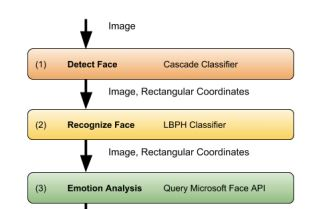
\includegraphics[width=\columnwidth]{Attendance_Emotion_1.JPG}}
\caption{Visual representation of this method.}
\label{Emotion1}
\end{figure}

A Cascade classifier is a classifier that is trained with thousands of positive and negative samples that are used to detect objects in other images \cite{b2}. In this situation, the positive example will be imaged with faces and the negative sample will be imaged without faces.

A Local Binary Patterns (LBP) combined with a Histogram of Oriented Gradients (HOG) creates LBPH which can be used for face recognition tasks. LBP is a simple yet very efficient texture operator that labels the pixels of an image by thresholding the neighborhood of each pixel and considers the result as a binary number. HOG is used to improve the detection performance considerably on some datasets.

\subsubsection{}Pros and Cons 

One of the advantages of this method is that it is relatively easy to learn for new coders. A beginner can learn the basic skills of face detection, face recognition, and emotional analysis \cite{b1}. Another advantage of this method is that it has a lot of potentials to grow; an example will be expanding this method to detect an unauthorized person.

One of the cons is that the accuracy of detecting a correct face is relatively low; there is a 40 percent accuracy; this might be caused by the distance that a camera is used when the picture is taken. Figure. \ref{Emotion2} shows an average score relate to this.  Another disadvantage of this Computer Vision for Attendance and Emotion Analysis in School Settings paper is that it has a small amount of dataset \cite{b1}. 

\begin{figure}[htbp]
\centerline{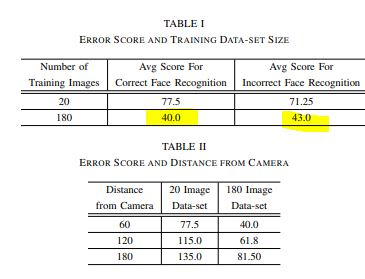
\includegraphics[width=\columnwidth]{Attendance_Emotion_2.JPG}}
\caption{Image of the Tables from this method.}
\label{Emotion2}
\end{figure}

% ===========================
% Automated Online Exam Proctoring
% ===========================

\subsection{Automated Online Exam Proctoring}
\subsubsection{}Why?

As we move to online learning, we need a way to automate online exams to avoid cheating as well as to minimize personnel resources.

\subsubsection{}How? 

The Automated Online Exam Proctoring paper talks about its multimedia analytics system to perform automatic and continuous online exam proctoring \cite{b3}.

This paper’s methods architecture has 3 main sections, the OEP Hardware, Basic Components, and Cheat Detection. In this survey, I will be only focusing on a portion of the cheat detection which uses Support Vector Machine (SVM) to detect the cheating behaviors. Figure. \ref{AOE1} shows the architecture of this paper.

\begin{figure}[htbp]
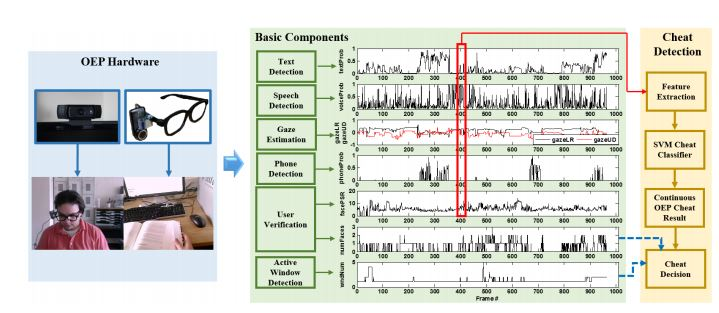
\includegraphics[width=\columnwidth]{AOE_1.JPG}
\caption{Architecture of the Automated Online Exam Proctoring Paper.}
\label{AOE1}
\end{figure}

SVM is a set of supervised learning methods most commonly used in classification, regression, and outliers detections \cite{b4}. The main idea is to represent a dataset as a set of points in space and separate them by categories that have a clear gap/distance from each category.

The Automated Online Exam Proctoring paper uses an SVM classifier to make continuous decisions on cheat behaviors. They divided their dataset into a positive class, cheating behaviors, and, negative class, non-cheating behaviors. They divided the positive class into 3 categories, text related cheating, speech cheating, and cheating using a phone \cite{b3}. 

\subsubsection{}Pros and Cons 

One of the advantages of this method is that is affordable and convenient to use from the test taker’s perspective as it only requires a couple of inexpensive camera and microphone, besides this, they have an accuracy of 87\% to detect cheating behaviors \cite{b3}.

One of the cons of this method is that is a little bit too complex; it consisted of various techniques besides computer vision.

% ===========================
% Controlling Mouse Motions Using Eye Tracking Using Computer Vision
% ===========================

\subsection{Controlling Mouse Motions Using Eye Tracking Using Computer Vision}
\subsubsection{}Why?

This paper talks about how to control/mimic a mouse motion using your face. I believe that this will be useful for educational purposes as students with disabilities; for example, not having hands; to use a computer in an online course.

\subsubsection{}How? 

The algorithm of this paper is made of three types of detection, Face detection, Eye Detection, and Mouth Detection \cite{b5}. 

For the face detection of this algorithm, the paper uses a pre-trained dataset iBug 300-Wand openCV to detect a face. For the eye detection section, the paper used the Eye-Aspect-Ratio (EAR) to determine whenever a person’s eye is flickering or not. Finally, for the mouth detection, they used the mouth-aspect-ratio (MAR) to determine whenever a mouth was opened or not.

To summarize, this paper uses a pre-trained dataset that maps facial coordinate points to a face; following this, it uses the EAR and MAR mathematical equations to determine the eyes and mouth movements. The EAR and MAR equations are shown in Figure. \ref{EAR} and Figure. \ref{MAR}

\begin{figure}[htbp]
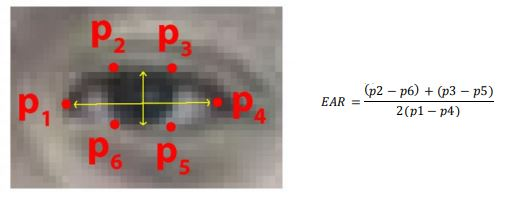
\includegraphics[width=\columnwidth]{EAR.JPG}
\caption{EAR Equation and Image of Eye Points.}
\label{EAR}
\end{figure}

\begin{figure}[htbp]
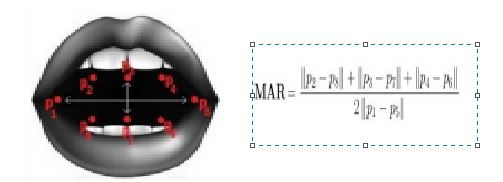
\includegraphics[width=\columnwidth]{MAR.JPG}
\caption{MAR Equation and Image of Mouths Points.}
\label{MAR}
\end{figure}
    
The algorithm used can be shown in Figure. \ref{FlowChart1}. The basic steps of the algorithm are the following.

\begin{figure}[htbp]
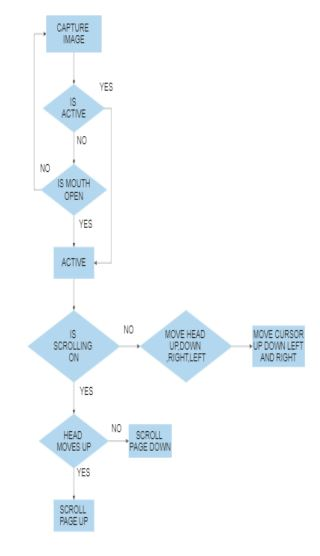
\includegraphics[width=\columnwidth]{FlowChar1.JPG}
\caption{FlowChar1 of the Algorithm.}
\label{FlowChart1}
\end{figure}

\begin{itemize}
    \item You have a camera that looks at a picture to detect a face.
    \item If it detects a face, it will decide what kind of eye or mouth movement the user is making.
    \item If a user wants to scroll a page, they will squint their eyes and move their face up and down.
    \item If they want to mimic a left or right-click of a mouse, they will squint the corresponding eye.
    \item They will open or close their mouth if they want to enable mouse control.
\end{itemize}

\subsubsection{}Pros and Cons 

An advantage of this method is that it uses basic concepts and resources for face detection, besides this, the dataset iBug 300-Wand is quite big as it has been created for competitions \cite{b6}.

A disadvantage of this paper is that it doesn’t tell us how accurate or the success rate of this algorithm; it just tells us that it showed correct results [4]. Another issue might be that the face detection might be inaccurate for some of the points for the EAR and MARS equation

% ===========================
% Detection & Identification of Human Body using FA based Algorithms
% ===========================

\subsection{Detection \& Identification of Human Body using FA based Algorithms}

\subsubsection{}Why?

We can use computer vision to detect the human body. This is useful in education as we can use this to detect unusual shapes or behavior by identifying human shapes.

\subsubsection{}How? 

This paper’s algorithm is divided into two sections. First, we have the Person Detection System which uses a Feature and Appearance (FA) Algorithm. Then we have the person recognition System that uses a Multiclass Support Vector Machine (MSVM) \cite{b7}. Figure x and y show the complete system for each section.

An MSVM is a regular SVM scaled to multiclass problems. More information and mathematical equations can be found in On the Algorithmic Implementation of Multiclass Kernel-based Vector Machines paper \cite{b8}.

\subsubsection{}Pros and Cons 

An advantage of this method is that it has a high accuracy for detecting the human body as shown in Figure. \ref{FA}.

\begin{figure}[htbp]
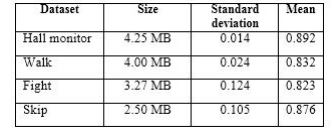
\includegraphics[width=\columnwidth]{Test1.JPG}
\caption{Accuracy for FA algorithm}
\label{FA}
\end{figure}


A disadvantage of this method or paper is that it doesn’t specify what type of feature and appearance algorithm it uses. It also uses a complex type of classifier, MSVM.

% ===========================
% Computer Vision Based Object Tracking as a Teaching Aid for High School Physics Experiments 
% ===========================

\subsection{Computer Vision Based Object Tracking as a Teaching Aid for High School Physics Experiments}

\subsubsection{}Why?

Computer Vision can also be used to enhance students learning ability by keeping them engaged. An example of this is in science education. As we know, experiments play a vital role in learning the material. In high school physics, especially in mechanics, many experiments are conducted where tracking a single or multiple objects are required. This manual method is time-consuming, generates a higher error, and incapable of producing multiple readings rapidly \cite{10}. This is where Computer Vision can be used to help students gather data easier and faster.

\subsubsection{}How? 

This paper’s methods have 5 main parts. First, we have image acquisition where we use a camera or any sort of device to take pictures or videos of an experiment. 

Following this, we have the Image preprocessing where they use Histogram equalization and they crop the image to include only the region of interest.

Next, we have the feature extraction where they use simple edge detectors such as the canny edge detector or the differential edge detector.

After this we have the object identification system where it uses different types of detectors such as Harris \cite{b11}, KLT \cite{b12}, and Moravec \cite{b13}.

Finally, they export the data, and students are enabled to use such data for their experiments. 

\begin{figure}[htbp]
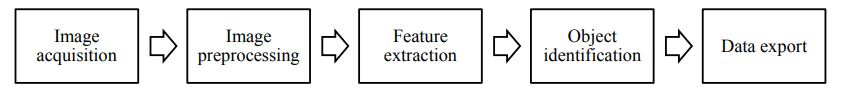
\includegraphics[width=\columnwidth]{FlowChar2.JPG}
\caption{FlowChart for Computer Vision in Experiments}
\label{FlowChart2}
\end{figure}

\subsubsection{}Pros and Cons 

Some advantages of this method include that it is flexible and can be changed depending on the experiment or situation. According to this paper, several standard high school physics experiments were conducted where computer vision-based tracking was used to aid the data gathering \cite{b10}. This proposed technique can be used to increase accuracy and to create new ways of conducting science experiments.

Figure. \ref{Track1} and Figure. \ref{Test2} shows a couple of graphs of data gathering that this method used for some experiments.

\begin{figure}[htbp]
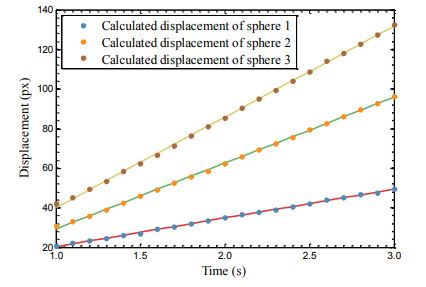
\includegraphics[width=\columnwidth]{Fig2.JPG}
\caption{Tracking a ball location against time}
\label{Track1}
\end{figure}

\begin{figure}[htbp]
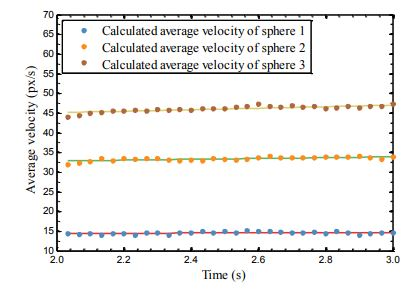
\includegraphics[width=\columnwidth]{Fig3.JPG}
\caption{Tracking an average terminal velocity of different size spheres}
\label{Test2}
\end{figure}

A disadvantage of this method is that it is too broad. As this method doesn’t specify what type of image preprocessing or feature detection; we will need to test various types of techniques to find the most optimal result for each experiment.

% ===========================
% Using Video to Automatically Detect Learner Affect in Computer-Enabled Classrooms
% ===========================

\subsection{Using Video to Automatically Detect Learner Affect in Computer-Enabled Classrooms}

\subsubsection{}Why?

During online lectures, it is really hard to see if a student is engaged or distracted from the lecture. Computer Vision can help detect students' effect from facial expression and gross body movements \cite{b14}. By detecting such effects, we can inform the instructor so that the instructor can do something about it.

\subsubsection{}How? 

This paper method uses FACET, a commercialized version of the CERT computer-vision software \cite{b14}. FACET is a program that is no longer publicly available that is used for facial feature extraction.
 
FACET gives a likelihood of facial movement such as Inner Brow Raise, Nose Wrinkle, and so on. Figure \ref{FACET} shows an example of the FACET program.

\begin{figure}[htbp]
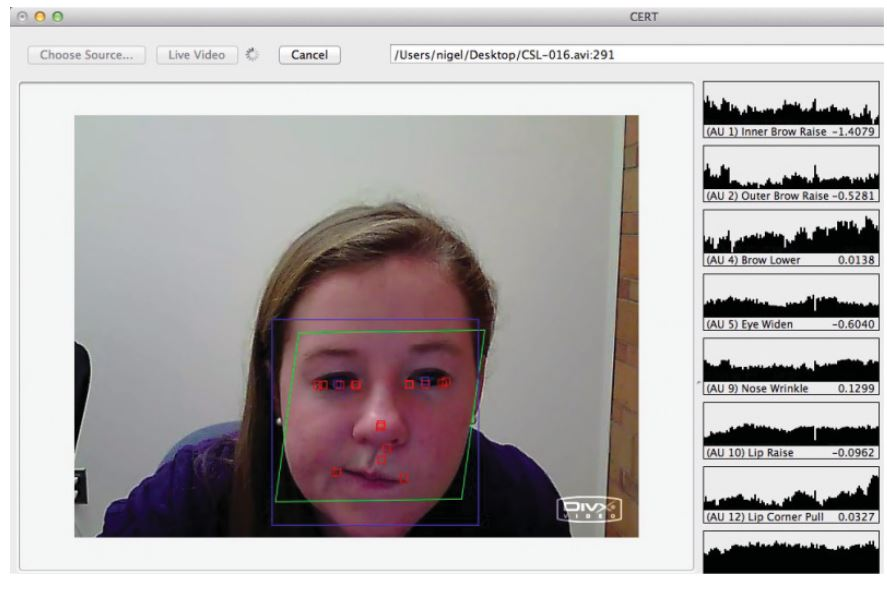
\includegraphics[width=\columnwidth]{FACET.JPG}
\caption{FACET program}
\label{FACET}
\end{figure}

To compute gross body movement, this paper by measuring the proportion of pixels in each video frame and see if there was a difference in each of them by a certain threshold.
 
Following this, they used a supervised learning method to calculate the emotion of a student, if they were bored, confused, happy, etc. They used 14 different classifiers such as Bayesian classifiers,
logistic regression, classification via clustering, and so on \cite{b14}.
 
Finally, they used Cross-validation for baseline classification, Figure. \ref{Table2} shows the result that this paper obtained.

\begin{figure}[htbp]
    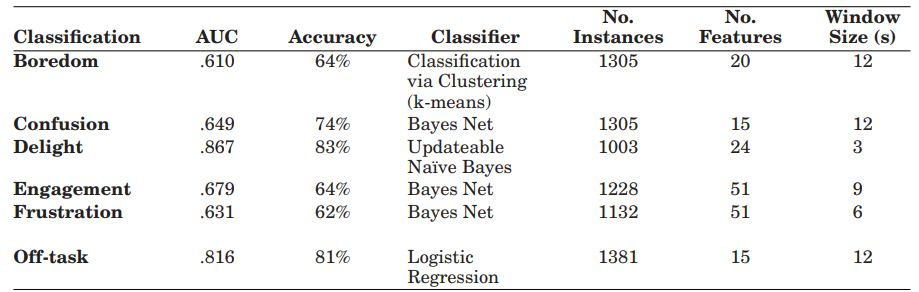
\includegraphics[width=\columnwidth]{Table2.JPG}
    \caption{Details and Results for Baseline Classification with All Data}
    \label{Table2}
    \end{figure}

\subsubsection{}Pros and Cons 

An advantage of this method is that is quite promising as it uses FACET for face recognition. 
 
A disadvantage of this method is the amount of data that we have to train the model as mentioned in the paper \cite{b14}. Another disadvantage might be the lighting conditions of the environment as it might affect the detection.
\subsection{Conclusion}

In this paper, we talked about different types of computer vision that we can use in education.

First of all, we talked about how to use computer vision for attendance and emotion analysis. We can use LBPH for face recognition and use Microsoft Face API to detect their emotions.

Following this, we talked about how we can automate online exam proctoring that uses SVM to make a continuous decision on cheat behaviors.

Next, we talked about using face recognition to help students with disabilities use a computer for educational purposes. It uses face recognition, EAR, and MAR equations to have a controlling mouse moving program using eye-tracking.

After this, we talked about how we can identify the Human body using feature and appearance algorithms. This algorithm uses a multiclass support vector machine and has a high accuracy for detecting.

Besides this, we talked about how computer vision can be used during classes. It can be used to enhance student data gathering for experiments or labs.
 
Finally, we talked about how we can use video to automatically detect the learner effect in computer-enabled classrooms. We learn that we can use FACET to help us do this detection.

We learn that we can use existing computer vision algorithms and apply them to education by tracking students’ behavior, helping students with disabilities, and more. Computer vision creates a new set of possibilities for education.

\begin{thebibliography}{00}
\bibitem{b9} A. Rosenfeld, "Computer vision: basic principles," in Proceedings of the IEEE, vol. 76, no. 8, pp. 863-868, Aug. 1988, doi: 10.1109/5.5961.
\bibitem{b1} S. Deniz et al., "Computer Vision for Attendance and Emotion Analysis in School Settings," 2019 IEEE 9th Annual Computing and Communication Workshop and Conference (CCWC), Las Vegas, NV, USA, 2019, pp. 0134-0139, doi: 10.1109/CCWC.2019.8666488.
\bibitem{b2} OpenCV, "Cascade Classifier Training", Dec 2020. Accessed on: Dec, 2020. [Online]. Available: https:\text{//}docs.opencv.org\text{/}3.4\text{/}dc\text{/}d88\text{/}tutorial\_traincascade.html
\bibitem{b3} Y. Atoum, L. Chen, A. X. Liu, S. D. H. Hsu and X. Liu, "Automated Online Exam Proctoring," in IEEE Transactions on Multimedia, vol. 19, no. 7, pp. 1609-1624, July 2017, doi: 10.1109/TMM.2017.2656064.
\bibitem{b4} Scikit-Learn, "1.4 Support Vector Machine". Accessed on: Dec, 2020. [Online]. Available: https:\text{//}scikit-learn.org/stable/modules/svm.html
\bibitem{b5} K. Meena, M. Kumar and M. Jangra, "Controlling Mouse Motions Using Eye Tracking Using Computer Vision," 2020 4th International Conference on Intelligent Computing and Control Systems (ICICCS), Madurai, India, 2020, pp. 1001-1005, doi: 10.1109/ICICCS48265.2020.9121137.
\bibitem{b6} iBug, "300 Faces In-The-Wild Challenge (300-W), IMAVIS 2014". Accessed on: Dec, 2020. [Online]. Available: https://ibug.doc.ic.ac.uk/resources/300\text{-}W\_IMAVIS.
\bibitem{b7} S. Upadhyaya and M. Sujatha, "Detection \& identification of human body using FA based algorithms," 2017 International Conference on Energy, Communication, Data Analytics and Soft Computing (ICECDS), Chennai, 2017, pp. 469-472, doi: 10.1109/ICECDS.2017.8390210.
\bibitem{b8} K. Crammer and Y. Singer. On the Algorithmic Implementation of Multi-class.
\bibitem{b10} G. D. Illeperuma and D. U. J. Sonnadara, "Computer vision based object tracking as a teaching aid for high school physics experiments," 2017 4th International Conference on Electrical Engineering, Computer Science and Informatics (EECSI), Yogyakarta, 2017, pp. 1-6, doi: 10.1109/EECSI.2017.8239112.
\bibitem{b11} K. Derpanis, The harris corner detector. 2004.
\bibitem{b12} Jianbo Shi and Tomasi, “Good features to track,” in Proceedings of IEEE Conference on Computer Vision and Pattern Recognition CVPR94, 1994, pp. 593–600.
\bibitem{b13} H. P. Moravec, “Rover visual obstacle avoidance,” Proc. 7th Int. Jt. Conf. Artif. Intell. IJCAI, vol. 2, pp. 785–790, 1981. 
\bibitem{b14} Nigel Bosch, Sidney K. D'mello, Jaclyn Ocumpaugh, Ryan S. Baker, and Valerie Shute. 2016. Using Video to Automatically Detect Learner Affect in Computer-Enabled Classrooms. <i>ACM Trans. Interact. Intell. Syst.</i> 6, 2, Article 17 (August 2016), 26 pages. DOI:https://doi-org.eres.library.manoa.hawaii.edu/10.1145/2946837
\end{thebibliography}
\vspace{12pt} 

\end{document}
